\documentclass[tikz,border=2pt]{standalone}
\usepackage{amsmath}
\usepackage{pgfplots}
\pgfplotsset{compat=1.18}
\usetikzlibrary{arrows.meta}
\begin{document}
% K=Cone({(1,0),(1,1)}) and its polar K°=Cone({(0,-1),(-1,1)}); each edge of K° is perpendicular to an edge of K.
% -K=Cone({(-1,0),(-1,-1)}) lies strictly inside K°, so K° is not -K.
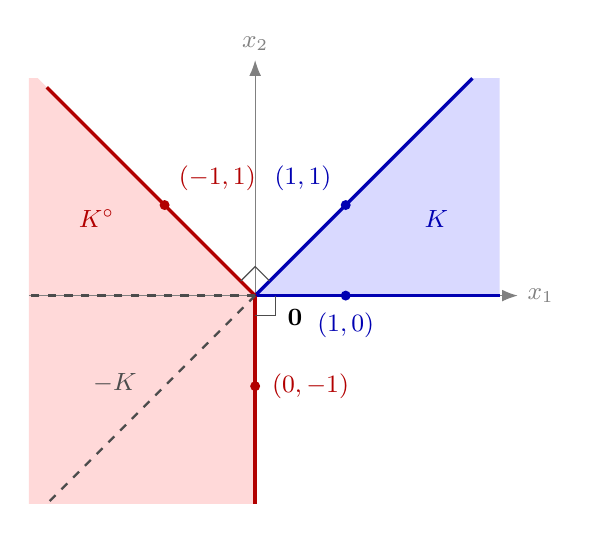
\begin{tikzpicture}[font=\small, >={Latex[length=2mm]}, x=1.15cm, y=1.15cm]
  \begin{scope}
    \clip (-2.5,-2.3) rectangle (2.7,2.4);
    \fill[blue!15] (0,0) -- (5,0) -- (5,5) -- cycle;
    \fill[red!15] (0,0) -- (-5,5) -- (-5,-5) -- (0,-5) -- cycle;
  \end{scope}
  \draw[gray, ->] (-2.5,0) -- (2.9,0) node[anchor=west] {$x_1$};
  \draw[gray, ->] (0,-2.3) -- (0,2.6) node[anchor=south] {$x_2$};
  \draw[blue!70!black, very thick] (0,0) -- (2.7,0);
  \draw[blue!70!black, very thick] (0,0) -- (2.4,2.4);
  \draw[red!70!black, very thick] (0,0) -- (0,-2.3);
  \draw[red!70!black, very thick] (0,0) -- (-2.3,2.3);
  \draw[gray!60!black, thick, dashed] (0,0) -- (-2.5,0);
  \draw[gray!60!black, thick, dashed] (0,0) -- (-2.3,-2.3);
  % right-angle marks
  \draw[gray!60!black] (0.22,0) -- (0.22,-0.22) -- (0,-0.22);
  \draw[gray!60!black] (0.16,0.16) -- (0,0.32) -- (-0.16,0.16);
  % generators
  \fill[blue!70!black] (1,0) circle (1.8pt);
  \node[blue!70!black, anchor=north] at (1,-0.08) {$(1,0)$};
  \fill[blue!70!black] (1,1) circle (1.8pt);
  \node[blue!70!black, anchor=south east] at (0.95,1.05) {$(1,1)$};
  \fill[red!70!black] (0,-1) circle (1.8pt);
  \node[red!70!black, anchor=west] at (0.08,-1) {$(0,-1)$};
  \fill[red!70!black] (-1,1) circle (1.8pt);
  \node[red!70!black, anchor=south west] at (-0.95,1.05) {$(-1,1)$};
  \node[blue!70!black] at (2.0,0.85) {$K$};
  \node[red!70!black] at (-1.75,0.85) {$K^{\circ}$};
  \node[gray!60!black, anchor=north] at (-1.55,-0.75) {$-K$};
  \node[anchor=north west] at (0.25,-0.04) {$\boldsymbol{0}$};
\end{tikzpicture}
\end{document}
